\subsection{Implementation Plan}
The TrackMe system will be implemented component by component, prioritizing the development of the most critical ones. Another key element on which the order of the implementation is decided is the level of dependency between components. This means that if multiple components depend on a single one then the development of the latter is prioritized upon the others, this way we can start integrating components as soon as they get developed and tested. Also it's considered good practice to concentrate first on the model part of the system, then to concentrate on the controller and last on the view.

The following tree contains components as nodes and is useful for describing the order of implementation from top to bottom following this rule: a node is implemented before its children.

\begin{figure}[H]
\centering
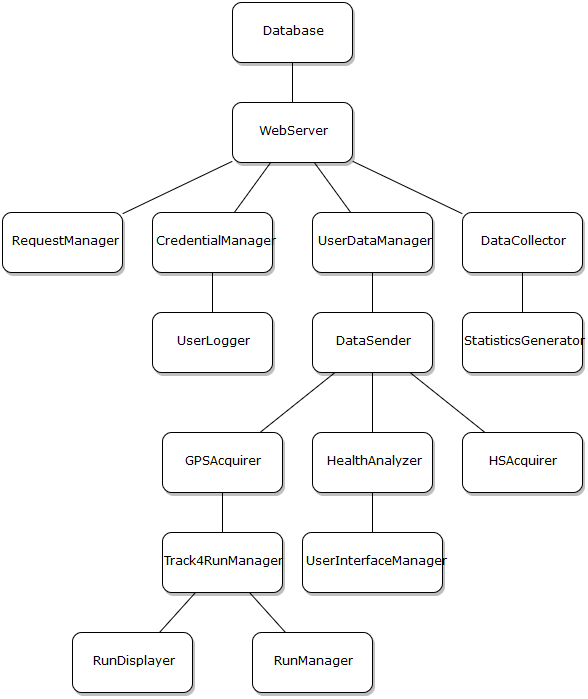
\includegraphics[scale=0.5]{Images/ImplementationPlan.png}
\caption{Implementation tree.}
\end{figure}

The first component that will be developed is the Database due to the fact that almost every component of our system will exploit Database's features, also it's one of the most critical parts of the system, if it fails then all our system will as well, and lastly it forms the model of our system.

The WebServer component will be developed right after the Database.



